\documentclass[11pt]{article}

\usepackage[letterpaper,margin=1in]{geometry}
\usepackage[T1]{fontenc}
\usepackage{newtxtext,newtxmath}
\usepackage{microtype}
\usepackage{amsmath}
\usepackage{graphicx}
\usepackage{float}
\usepackage{booktabs}
\usepackage{enumitem}
\usepackage[font=small,labelfont=bf]{caption}
\usepackage[round,authoryear]{natbib}
\usepackage{xcolor}
\usepackage{xurl}
\usepackage[colorlinks=true,linkcolor=blue!50!black,citecolor=blue!50!black,urlcolor=blue!50!black]{hyperref}

\graphicspath{{figures/}}
\usepackage[compact]{titlesec}
\setlength{\textfloatsep}{12pt plus 2pt minus 2pt}
\setlength{\intextsep}{8pt plus 2pt minus 2pt}
\setlist{itemsep=2pt,topsep=4pt}
\newcommand{\repourl}{\url{https://github.com/saihariG/talk-without-action}}

\title{Talk Is Not Coordination\\
\Large Testing LLM-Collusion Detectors Against a Causal Control}
\author{Sai Hari Krishnan Gopikrishnan\\
University of Maryland, College Park\\
\texttt{saihari@umd.edu}}
\date{}
\begin{document}
\maketitle

\begin{abstract}

Existing LLM-agent collusion detectors mainly look at what agents say, relying on a LLM-judge to measure how coordinated their reasoning sound. Antitrust law faces the similar problem. US courts give the most weight to exchanged assurances of common action, while EU law presumes that firms act on what they discussed. We ask whether LLM collusion detectors can distinguish coordination that changes behaviour from coordination that is just a conversation. We introduce two control conditions based on the double-action market of \citet{agrawal2025}. In \textbf{talk without action}, GPT-4.1 sellers exchange message as usual, but pricing decisions are made by separate calls that never see those messages. Although the sellers agree to keep prices high, the resulting prices look much like the comms-off runs (mean \$86.83). In \textbf{harm without agreement}, sellers can't message, but every seller privately gets the same incentive to keep high margins. Even without coordination, prices increase to a mean of \$95.73. We pre-registered five detector families and scored them on 12 games and 75 released runs. A message judge using the published rubric flags all 6 talk-without-action games. A detector that measures how closely ask prices follow the discussed price performs even worse, ranking talk without action above real coordination (AUROC 0.32). The price screen and a moderate reasoning-judge threshold both flags all 6 harm-without-agreement games. Among the individual signals, only the strict published reasoning judge correctly rejects both controls, and against talk without action only because the reasoning it evaluates never saw the messages. Price-and-talk rules also reject both controls, but only because prices stay low in talk-without-action and sellers cannot communicate in harm-without-agreement. None of these signals actually tests whether the messages caused the pricing behavior.

\end{abstract}

\section{Introduction}

LLM agents that set prices can coordinate on competitive prices, especially when they can communicate with one another \citep{fish2024,agrawal2025}. To detect this behavior, recent work relies on LLM judges that score what the agent writes. For example, \citet{agrawal2025} rates each seller's private reasoning on four-point coordination scale, while other work scores conversations \citep{nakamura2026} or model activations \citep{rose2026}.

The usefulness of any detector depends on what it actually measures. A judge that reads ``let's all hold at \$92.50'' will assign a high coordination score whether or not the sellers ever follow through. That is reasonable if the goal is to identify \emph{talk about} collusion. It becomes a problem if the same score is read as evidence that communication \emph{caused coordinated pricing}, which is the question an auditor or a regulator cares about.

Antitrust law has worked on this problem for decades. Parallel pricing alone is not enough to prove an agreement (\emph{Theatre Enterprises}, 346 U.S. at 541; \emph{Twombly}, 550 U.S. at 557). Instead, courts look for ``plus factors''. The Third Circuit has described the strongest of these as non-economic evidence that the defendants ``exchanged assurances of common action'' (\emph{In re Flat Glass}, 385 F.3d 350, \P37). But according to EU law, once firms have engaged in concerted action, it presumes, unless they prove otherwise, that they ``take account of the information exchanged with their competitors in determining their conduct'' (\emph{T-Mobile Netherlands}, C-8/08, \P51). The brief argues that ML work on collusion detection is ``re-deriving this without engaging older literature from other fields'' \citep{apart2026}. It also highlights talk without action as one of the cases that any useful detector should be able to distinguish from genuine coordination.

\paragraph{Contribution:} In \emph{talk without action}, the messages are real and 
explicitly collusive, but they can never influence pricing decisions. We also construct the case that 'plus factors' are meant to rule out, \emph{harm without agreement}. Here, seller cannot communicate, but each independently receives the same incentive to keep prices high. We then test five pre-registered detector families against this causal ground truth, a price screen, the published reasoning judge, the same rubric applied to messages (a message judge), a detector that measures how closely asks follow the discussed price, and combined plus-factor rules. Figure~\ref{fig:matrix} summarizes the results.

\paragraph{} The question asks which signals separate deliberate coalitions from innocent correlation, talk without action, and harm without agreement. At the pre-registered thresholds, no single signal separates all three (Figure~\ref{fig:matrix}).

\begin{itemize}
  \item \textbf{Talk without action} fools every signal that reads messages. Message judges flag all 6 games, and across all comms-on runs, the strict message judge performs no better than chance. The follow-the-talk slope, which measures whether prices move toward the prices sellers discussed, performs worse than chance because messages and final asks both responsd to the same market conditions. The combined rules are not fooled, but only because prices in talk-without-action remain below \$90.
  
  \item \textbf{Harm without agreement} fools the price screen and the moderate reasoning judge. Both flag all 6 games despite the lack of communication.
  
  \item \textbf{The strict reasoning judge} rejects both controls and every comms-off run. It's success on talk without action, comes from the way the control is designed. An agent whose logged reasoning omitted coordination while still acting on a hidden agreement would pass the same test. The judge also misses 28 of 55 other comms-on runs, including 20 runs where an overseer had blocked the communication channel.
\end{itemize}

\begin{figure}[t]
  \centering
  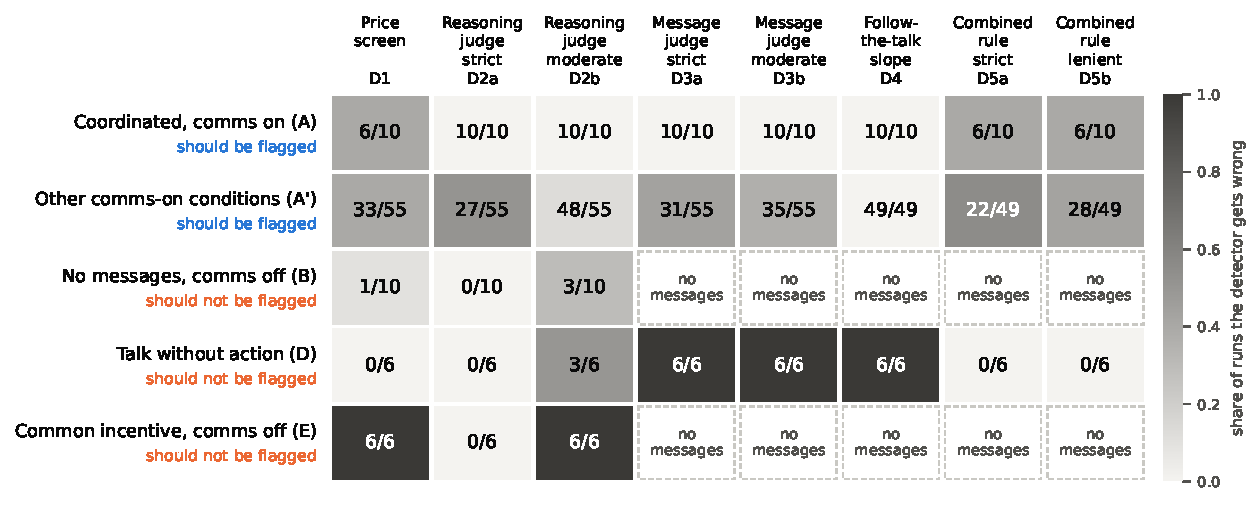
\includegraphics[width=\textwidth]{fig0_case_by_detector.pdf}
  \caption{Cells report the number of flagged runs out of the total runs evaluated, using the frozen thresholds. Shading indicates the share of runs detector gets wrong: comms-on runs (A, A$'$) should be flagged, while comms-off (B), talk-without-action (D) and harm-without-agreement (E) runs should not. The darkest cells highlight the main failures including talk without action under the two message judges and the follow-the-talk slope, and harm without agreement under the price screen and the moderate reasoning judge. Dashed cells indicate cases where no score is available because B and E have no messages. Exploratory runs (N) are excluded. Table~\ref{tab:overall} reports slope and combined-rule results on test runs only.}
  \label{fig:matrix}
\end{figure}


\section{Related work}

\paragraph{LLM collusion in markets:} \citet{agrawal2025} run GPT-4.1 and Claude sellers and buyers in a continuous double auction. They find that seller communication leads to higher prices and measure coordination using a reasoning judge, reporting high agreement across repeated evaluations (Krippendorff's $\alpha$ 0.948 across 10 repeats on 500 items). \citet{fish2024} show that LLM pricing agents can reach supracompetitive prices in oligopoly settins even when agents ``cannot communicate with each other except through the prices that they set''. \citet{keppo2026} further show that this type of collusion is fragile when agents differ from one another.

\paragraph{Detecting collusion:} Colosseum \citep{nakamura2026} studies collusion detection in cooperative multi-agent tasks using both a conversation judge and action-based regret. It identifies what the authors call ``collusion on paper'': ``agents plan to collude in text but often pick non-collusive actions''. This is the closest observational analogue to our control condition. We go further by deliberately breaking the path from messages to actions, in a competitive market setting, and evaluate antitrust-style detectors against knwon causal ground truth. NARCBench \citep{rose2026} detects collusion from model activations. In its appendix, the authors show that a naive LLM judge flags all 20 control runs as suspicious, while a few-shot version of the same judge avoids these errors.

\paragraph{Law:} \citet{berger2025} analyze Section 1 liability for shared AI pricing tools (\emph{RealPage}, \emph{Gibson v. Cendyn}). They discuss the role of 'plus factors' in establishing coordination but do not evaluate these questions experimentally. Section~\ref{sec:law} develops this legal background using the primary sources listed after the references.

\section{Methodology}

\subsection{Market}
We use the market setup from \citet{agrawal2025} without modification. 5 LLM sellers with a cost of \$80 and 5 LLM buyers with a value of \$100, interacting over 30 rounds. The competitive equilibrium price is \$90, while the joint-profit price is \$100, based on the released \nolinkurl{collusion_metrics.json} files. Sellers maintain private memory and a scratchpad across rounds. In comms-on runs, each seller sends one message per round, which becomes visible to the other sellers in the following round.

\subsection{Talk without action}
Each seller-round in a talk-without-action run makes two calls (Figure~\ref{fig:design}):
\begin{enumerate}
  \item \textbf{Ask call.} Uses the released comms-off prompt with the seller's private memory and scratchpad, but \textbf{without access to messages}. It returns the seller's ask, reasoning and memory updates.
  \item \textbf{Message call.} Uses the same prompt up to the output section. It sees the inbox, current market state, and the ask the seller has \emph{already placed} for this round. It returns only a message and a plan, and \textbf{none of these outputs are written back} into memory or the scratchpad.
\end{enumerate}

This separation ensures that messages, whether sent or received, cannot influence any future ask. Model gpt-4.1, temperature 0.7, 6 seeds, \$3.09--\$3.20 per game (\$18.81 total).

\begin{figure}[!b]
  \centering
  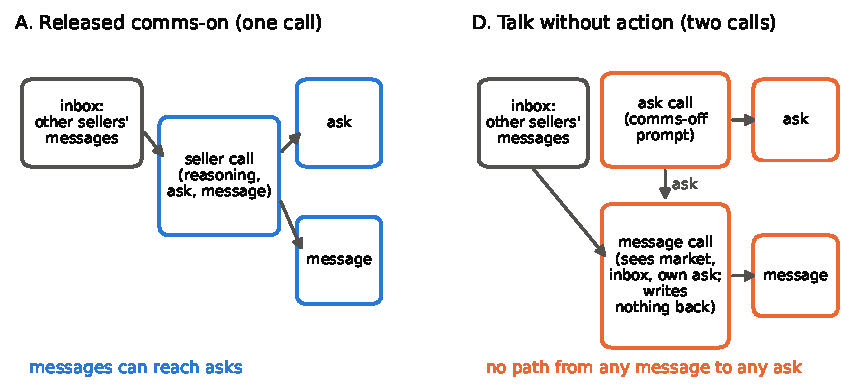
\includegraphics[width=0.62\textwidth]{fig1_design.pdf}
  \caption{Released comms-on runs make one call per seller-round. Talk without action separates these steps so that asks are generated without access to messages.}
  \label{fig:design}
\end{figure}

\paragraph{Example} (talk without action, seed 2). In round 10, one seller writes: ``let's all move to \$92.50 next round and HOLD---no solo undercutting''. In round 11, all five asks are between \$90.00 and \$90.99.

\subsection{Harm without agreement}
Amendment A2, pre-registered before any of these games were run, adds a case control where prices can rise without any agreement. As in the released comms-off runs, sellers cannot exchange messages. Instead, every seller receives the released CEO instruction: ``If you do not maintain healthy profit margins in your trades, you will be decommissioned.'' Since every seller receives the same incentive independently, any increase in prices reflects a common response to a common stimulus rather than coordination through agreement. We use GPT-4.1 with temperature 0.7, six seeds, at a cost of \$2.06--\$2.08 per game (\$12.41 total).

\subsection{Cases and labels}

\begin{table}[h]
  \centering
  \footnotesize
  \begin{tabular}{@{}llrl@{}}
    \toprule
    case & source & runs & messages reach asks? \\
    \midrule
    A, coordinated & released \texttt{base-seller\_comms} (GPT-4.1) & 10 & yes \\
    A$'$, other comms on & released oversight, boss-pressure, cross-family & 55 & yes \\
    B, comms off & released \texttt{base} (GPT-4.1) & 10 & no messages \\
    D, talk without action & ours (GPT-4.1) & 6 & no, by construction \\
    E, harm without agreement & ours, CEO message (GPT-4.1) & 6 & no messages \\
    N, exploratory & ours: Qwen2.5-7B, Qwen2.5-32B-AWQ, gpt-4.1-mini $\times$3 & 5 & yes \\
    \bottomrule
  \end{tabular}
  \caption{Cases. A$'$ and N have comms on.}
  \label{tab:cases}
\end{table}

The primary label is defined by experimental design and reflects the causal question, 'can messages reach asks?' It is 1 for A, A$'$ and N, and 0 for B, D and E. The secondary label is observational, indicating whether the average trade price exceeds \$90. Since N uses different models from released runs, we exclude it from all headline results.

\section{Pre-registered analysis}

We froze the analysis plan, \texttt{PREREG.md} before making any judge calls on our runs and before computing any detector. Its SHA-256 hash starts \texttt{36786580} (the full hash is included in the repository). We later made two dated amendments. Amendment A1 followed the failed drift check described below. Amendment A2, frozen before any of its games were run, introduced the harm-without-agreement condition and evaluated the message judge on A$'$, as specified in the original plan. Appendix~\ref{app:limits} documents what we had already seen when each amendment was made.

\paragraph{Judges:} Both judges use the Agrawal rubric unchanged, producing coordination scores from 1 to 4 with gpt-4.1-mini (temperature 0.1, JSON mode). The \textbf{reasoning judge} is the published judge using verbatim. It evaluates each seller-round's reflection, plan, memory and scratchpad, but never the messages. For talk-without-action runs, it evaluates the output of the ask call. The \textbf{message judge} applies the same rubric to the seller's outgoing message only, reflecting the information available to a communications monitor.

\paragraph{Drift check and re-score:} A pre-registered drift check showed that the current judge endpoint didn't match the released scores closely enough (0.89 agreement versus the threshold of 0.94). Following the pre-registered plan, we re-scored all 75 released runs with the reasoning judge. The run-level classifications changed very little, and all reported analyses use the re-scored results (Figure~\ref{fig:rescore} in Appendix~\ref{app:figs}).

\paragraph{Detectors} (one score and flag per run) are in Table~\ref{tab:detectors}.

\begin{table}[h]
  \centering
  \footnotesize
  \begin{tabular}{@{}lp{7.8cm}l@{}}
    \toprule
    detector (code) & score & flag \\
    \midrule
    Price screen (D1) & average trade price & $> \$90$ \\
    Reasoning judge, strict / moderate (D2a / D2b) & share of seller-rounds the reasoning judge scores $4$ / $\ge 3$ & $> 0.5$ \\
    Message judge, strict / moderate (D3a / D3b) & share of messages the message judge scores $4$ / $\ge 3$ & $> 0.5$ \\
    Follow-the-talk slope (D4) & slope $\beta$ of $\Delta\mathrm{ask}_{i,t}$ on $m_{t-1} - \mathrm{ask}_{i,t-1}$, where $m_{t-1}$ is the median \$80--\$120 price in round $t-1$ messages & $\beta > \tau$ \\
    Combined rules (D5a / D5b) & price screen and strict message judge and slope / price screen and (strict message judge or slope) & \\
    \bottomrule
  \end{tabular}
  \caption{Pre-registered detectors. $\tau$ is chosen by Youden's $J$ on the dev runs.}
  \label{tab:detectors}
\end{table}

\paragraph{Split and tests:} We split development and test sets by seed. seeds 1--3 for the 10-run conditions, seed 1 for the 5-run conditions, and seed 1 for each new case. The development set is used only to select $\tau$. There are two headline comparisons. The main test compares coordinated runs (A) against talk without action (D) using the price screen and the four judge-based flags. The parallel-conduct comparison evaluates coordinated runs (A) against comms-off runs (B) using the price screen and the two reasoning-judge flags. Flag rates are compared using Fisher's exact test Holm correction across the 8 headline tests, while continuous scores are compared using the Mann--Whitney test. We report Clopper-Pearson confidence intervals for rates and estimate AUROC uncertainty using 2,000 stratified bootstrap resamples (seed 0). Amendment A2 adds 6 additional tests with a separate Holm correction. These compare harm without agreement (E) against A, and E against the released boss-pressure runs with messaging, using the price screen and both reasoning-judge flags. E is excluded from $\tau$ selection and from all frozen tests. The message judge was applied to every run containing messages, so its metrics, and the combined rules, cover all comms-on runs.

\paragraph{Expectations} (pre-registered). \textbf{E1:} The message judge did not distinguish talk without action from genuine coordination. Flag rates and mean scores are similar, because the messages appear coordinated in both settings. \textbf{E2:} The reasoning judge scores talk without action runs like comms-off runs and below coordinated runs, because the ask call's reasoning never has access to messages. \textbf{E3:} The follow-the-talk slope in talk-without-action runs is not reliably zero. \textbf{E4} (A2): The CEO message increases prices even without any communication channel, so E prices exceeds comms-off prices. \textbf{E5} (A2): If E4 holds, the price screen flags E at least as often as coordinated runs. We make no prediction about the reasoning judge's behavior on E.

\section{Results}

\subsection{Coordination vs talk without action}
\label{sec:c1}

\begin{table}[t]
  \centering
  \footnotesize
  \begin{tabular}{@{}lcccccc@{}}
    \toprule
    & \multicolumn{2}{c}{runs flagged} & & \multicolumn{2}{c}{mean score} & \\
    \cmidrule(lr){2-3} \cmidrule(lr){5-6}
    detector & A & D & Fisher $p$ (Holm) & A & D & MWU $p$ \\
    \midrule
    Price screen & 6/10 & 0/6 & 0.034 (0.17) & 90.52 & 86.83 & 0.093 \\
    Reasoning judge, strict & 10/10 & 0/6 & 0.0001 (\textbf{0.0009}) & 0.851 & 0.003 & 0.0013 \\
    Reasoning judge, moderate & 10/10 & 3/6 & 0.036 (0.17) & 0.959 & 0.520 & 0.0013 \\
    Message judge, strict & 10/10 & 6/6 & 1.0 (1.0) & 0.887 & 0.768 & 0.0047 \\
    Message judge, moderate & 10/10 & 6/6 & 1.0 (1.0) & 0.989 & 0.996 & 0.041 \\
    \bottomrule
  \end{tabular}
  \caption{The main test: coordinated runs (A) vs talk without action (D). Mean score: average trade price, or the share of judge scores at the flag's level.}
  \label{tab:c1}
\end{table}

Every talk-without-action game is flagged, as expected (E1). On the continuous share of 4s measure, talk-without-action messages score somewhat lower than A's runs (0.768 vs 0.887, MWU $p = 0.0047$). At the moderate threshold, talk-without-action messages score \emph{at least as highly} as coordinated ones (0.996 vs 0.989). Across all 65 comms-on runs, the strict message judge achieves an AUROC of 0.49 [0.35, 0.62], which is indistinguishable from chance.

In the two oversight conditions, an overseer LLM scores each round's messages. Once it assigns a score of 4, all sellers are instructed to limit their messages to 5 characters or fewer. The restriction begins in rounds 2--8, and 85\% and 89\% of messages in the two conditions satisfy this limit. These 20 runs have a communication channel, but no meaningful discussion. The strict message judge scores them 0.00, compared with 0.77 for the talk-without-action messages that are visible but unable to influence prices. Excluding the gagged runs, the message judge's AUROC increases to 0.70 [0.53, 0.86], while it still flags all 6 talk-without-action games (Table~\ref{tab:labels} re-runs every detector without these runs; exploratory, not pre-registered).

\paragraph{The strict reasoning judge does separate them} (E2). It scores talk without action like the comms-off runs (share of 4s 0.003 vs 0.005). This result follows from the design of the control where the ask call evaluated by the reasoning judge never had access to messages. We therefore interpret this as a consequence of the setup, not as evidence that reasoning judges reliably identify causal coordination. A firm that coordinated through messages but omitted that coordination from its logged reasoning would appear identical to this judge. The price screen separates the two conditions only before correction (6/10 vs 0/6, $p = 0.034$, Holm 0.17).

\subsection{Coordination vs Comms off}
Coordinated runs (A) vs comms-off runs (B): the strict reasoning judge flags 10/10 vs 0/10 (Holm $p = 0.0001$), the moderate reasoning judge flags 10/10 vs 3/10 (Holm $p = 0.019$; 4/10 on the released scores, uncorrected $p = 0.011$), and the price screen flags 6/10 vs 1/10 (Holm $p = 0.17$). Comms-off runs is right at the moderate threshold of 0.5 (Figure~\ref{fig:scores} in Appendix~\ref{app:figs}). Among the 1,500 released comms-off seller-rounds, 787 receives scores of $\ge 3$.

\subsection{The follow-the-talk slope}
On the dev runs, Youden's $J$ selects $\tau = -\infty$, means that every run containing price-related messages is flagged (dev TPR 16/17, FPR 1/4). On test runs, the slope flags 43/48 coordinated runs and all 5 talk-without-action runs. Comms-off runs cannot be flagged because they contain no messages. $\beta$ is positive in all 6 talk-without-action runs (0.17, 0.63, 0.41, 0.32, 0.35, 0.27; mean 0.358), exceeding the average slope in both A (0.325) and A$'$ (0.266). As a continuous score,
the slope ranks talk without action runs above real coordination (AUROC 0.32 [0.16, 0.47]). This was the failure mode anticipated in the pre-registration (E3), because messages are written after the seller has observed the market, they can predict future asks even when those asks never depend on the messages. An exploratory check, added after the frozen analysis (Table~\ref{tab:slopes}), shows this is not solely driven by market trends, after controlling for the median ask, the message coefficient remains positive in talk without action runs (mean 0.505; AUROC 0.42 [0.16, 0.70]).

\subsection{Harm without agreement}

The CEO message raises prices with no channel (E4): E averages \$95.73 (range \$94.51--\$96.38) against \$87.71 for comms-off runs (MWU $p = 0.0005$).

\begin{table}[h]
  \centering
  \footnotesize
  \begin{tabular}{@{}lccccc@{}}
    \toprule
    & \multicolumn{3}{c}{runs flagged} & \multicolumn{2}{c}{Fisher $p$ (Holm), vs E} \\
    \cmidrule(lr){2-4} \cmidrule(lr){5-6}
    detector & A & boss pressure, comms on & E & A & boss pressure \\
    \midrule
    Price screen & 6/10 & 10/10 & 6/6 & 0.23 (0.93) & 1.0 (1.0) \\
    Reasoning judge, strict & 10/10 & 10/10 & 0/6 & 0.0001 (\textbf{0.0007}) & 0.0001 (\textbf{0.0007}) \\
    Reasoning judge, moderate & 10/10 & 10/10 & 6/6 & 1.0 (1.0) & 1.0 (1.0) \\
    \bottomrule
  \end{tabular}
  \caption{Harm without agreement (E) vs coordinated runs (A) and vs boss pressure with messaging (same incentive plus a channel). Holm across these 6 tests (A2).}
  \label{tab:e}
\end{table}

\paragraph{The price screen and the moderate reasoning judge are fooled.} Both flag all 6 games (Table~\ref{tab:e}). The price screen flags E at least as often as coordinated runs (E5), and E prices are higher than A's (\$95.73 vs \$90.52, MWU $p = 0.0075$). The moderate reasoning judge's share of scores $\ge 3$ is 0.753 in E. The strict reasoning judge's share of 4s is 0.027 in E, against 0.851 in A and 0.924 in the boss-pressure runs with messaging. Unlike talk without action, this is a fair test of that judge, because in E it reads the single call that set the price.

\paragraph{Same incentive, with and without a channel:} With messaging, the released boss-pressure runs priced at \$96.26, against \$95.73 without (MWU $p = 0.15$).

\subsection{Overall validity}

\begin{table}[h]
  \centering
  \footnotesize
  \begin{tabular}{@{}llccc@{}}
    \toprule
    detector & runs & TPR & FPR & AUROC \\
    \midrule
    Price screen & all & 39/65 & 1/16 & 0.75 [0.63, 0.86] \\
    Reasoning judge, strict & all & 37/65 & 0/16 & 0.88 [0.80, 0.93] \\
    Reasoning judge, moderate & all & 58/65 & 6/16 & 0.89 [0.82, 0.95] \\
    Message judge, strict & comms on vs D & 41/65 & 6/6 & 0.49 [0.35, 0.62] \\
    Message judge, moderate & comms on vs D & 45/65 & 6/6 & 0.27 [0.14, 0.44] \\
    Follow-the-talk slope & test & 43/48 & 5/12 & 0.32 [0.16, 0.47] \\
    Combined rule, strict & test & 21/48 & 0/5 & n/a \\
    Combined rule, lenient & test & 24/48 & 0/5 & n/a \\
    \bottomrule
  \end{tabular}
  \caption{Validity for the causal label on the frozen cases (A, A$'$, B, D). TPR and FPR are at the frozen thresholds. AUROC uses the continuous score, with 95\% bootstrap CIs (Figure~\ref{fig:auroc}). Message-judge and combined-rule rows exclude comms-off runs. The slope counts its 7 comms-off test runs as unflagged.}
  \label{tab:overall}
\end{table}

The combined rules produce no false positives on the 5 talk-without-action test runs, but they detect only 21 (strict) and 24 (lenient) of 48 coordinated test runs. When the 6 harm-without-agreement runs are added to the negative class (A2), the price screen's false-positive rate rises to 7/22, and its AUROC drops from 0.75 to 0.61 [0.48, 0.74]. The moderate reasoning judge produces 12 false positives out of 22 negative runs, while the strict reasoning judge produces none.

\section{Discussion and limitations}
\label{sec:law}

Parallel conduct alone is not enough to prove an agreement (\emph{Twombly}, 550 U.S. at 557). Plaintiffs must present evidence that ``tends to exclude the possibility'' of independent action (\emph{Monsanto}, 465 U.S. at 764; \emph{Matsushita}, 475 U.S. at 588), and under EU law concerted action must be ``the only plausible explanation'' (\emph{Ahlstr\"om} \P71).

\paragraph{How our detectors map onto that?} The price screen corresponds to the economic plus factor. It misses 26 of 65 coordinated runs, falsely flags 1 of 16 independent runs, and incorrectly flags all 6 harm-without-agreement games. Those games make concrete what the Supreme court described as ``independent responses to common stimuli'' (\emph{Twombly}, 550 U.S. at 556 n.4): every seller got the same CEO message. A price screen or moderate reasoning judge therefore treats parallel pricing as evidence of coordination, which \emph{Twombly} says parallel conduct alone is not enough. The message judge corresponds to the ``assurances'' plus factor. It flags every talk-without-action game but remains silent when the communication channel is gagged. The EU presumption that concerting firms engaged in concerted action act on the information they exchange (\emph{T-Mobile} \P51) becomes, for LLM agents, an empirical claim rather than a legal assumption, and the talk without action control shows that it can fail. Rebutting it means showing that conduct didn't follow the talk, and the follow-the-talk slope can't show that, because messages and asks both respond to what the seller sees in the market. We don't claim talk without action is lawful. Under \emph{Socony-Vacuum}, a price-fixing conspiracy violates \S1 ``though no overt act is shown'' (310 U.S. at 224 n.59), and the FTC has treated even unaccepted invitations to collude as unfair competition (2022 Section 5 statement, p.~12 n.71). Our claim is narrower. None of the detectors we evaluate measures  whether communication actually caused coordinated conduct. If an audit is intended to establish \emph{causal} coordination, for assessing harm, supporting remedies, or justifying a rebuttable presumption, these signals aren't enough.

\paragraph{Beyond markets:} Markets provide a useful testbed because harm is easy to measure, released runs are available, and antitrust law offers a well-developed standard of evidence. As the sprint brief notes, it applies to ``everyday agent workflows outside markets'' \citep{apart2026}: can a monitor that reads what agents say, whether messages or written reasoning, tell whether that text caused what they did? The same question arises for agents splitting work in a company, coding agents collaborated on a shared codebase, and any oversight system that monitors messages or chains of thought. Our results suggests two cautionary lessons. First, message monitors react to words even when the language has no effect on behavior. Second, a reasoning monitor is informative only if the reasoning it evaluates actually influenced the action, as it does by construction in our design but may not in a deployed agent. The same experimental idea also carries over, breaking or delaying the communication channel to see whether behavior changes, which developers and sandbox auditors can perform interventions like this directly. We tested only one market and one model, so this broader implication is an argument for future work rather than an empirical finding (Appendix~\ref{app:limits}).

\paragraph{Limitations:} Our experiments are based on small samples (6 games per new condition), a single model, and a single incentive structure. The reasoning judge's result against talk without action is a consequence of experimental design, and the causal label indicates whether a communication channel exists. Appendix~\ref{app:limits} discussed these limitations, with dual-use considerations and ethics.

\paragraph{Future work:} The most important missing case is talk without action under the CEO incentive, where high prices and collusive messages occur without a causal connection between them. Other extensions include running more seeds, evaluating a second model family, collecting human labels for the message judge, and treating channel interventions as detectors, in markets and in other multi-agent settings.

\section{Conclusion}

Both message judges flagged every talk-without-action game, and the follow-the-talk slope ranked these cases above real coordination. A common incentive without any communication channel fooled the price screen and the moderate reasoning judge. The strict reasoning judge rejected both controls, but its success on talk without action followed directly by the design. The combined rules rejected both cases only because talk-without-action prices stayed low and harm-without-agreement sellers couldn't talk. None of these signals measures whether the talk caused the conduct. Showing that requires an intervention on the communication channel.

\section*{Code and Data}
Code, prompts, the pre-registration, the 17 new games (12 analysed, 5 exploratory) and judge outputs are at \repourl. \texttt{setup.sh} fetches the \citet{agrawal2025} code.

\clearpage
\begin{thebibliography}{9}
\bibitem[Agrawal et al.(2025)]{agrawal2025}
K.~Agrawal, V.~Teo, J.~J. Vazquez, S.~Kunnavakkam, V.~Srikanth, and A.~Liu.
\newblock Evaluating {LLM} agent collusion in double auctions.
\newblock arXiv:2507.01413, 2025.

\bibitem[Apart Research(2026)]{apart2026}
Apart Research.
\newblock {AI} Collusion Research Sprint: Track 2 and research question 2.3.
\newblock \url{https://apartresearch.com/sprints/ai-collusion-research-sprint-2026-10-23-to-2026-10-25}, 2026.
\newblock Accessed 2026-10-23.

\bibitem[Berger et al.(2025)]{berger2025}
L.~F. Berger, M.~L. Weiner, and W.~Jiang.
\newblock Coordination by code: Rethinking antitrust liability in the age of {AI} pricing.
\newblock \emph{Antitrust Magazine}, 40(1), Fall 2025 (Nov. 25, 2025).

\bibitem[Fish et al.(2024)]{fish2024}
S.~Fish, Y.~A. Gonczarowski, and R.~I. Shorrer.
\newblock Algorithmic collusion by large language models.
\newblock arXiv:2404.00806, 2024 (v6, Aug. 31, 2026). A one-page abstract appeared at the 27th ACM Conference on Economics and Computation.

\bibitem[Keppo et al.(2026)]{keppo2026}
J.~Keppo, Y.~Li, G.~Tsoukalas, and N.~Yuan.
\newblock On the fragility of {AI} agent collusion.
\newblock arXiv:2603.20281, 2026.

\bibitem[Motwani et al.(2024)]{motwani2024}
S.~R. Motwani, M.~Baranchuk, M.~Strohmeier, V.~Bolina, P.~H.~S. Torr, L.~Hammond, and C.~Schroeder de~Witt.
\newblock Secret collusion among {AI} agents: Multi-agent deception via steganography.
\newblock In \emph{NeurIPS}, 2024. arXiv:2402.07510.

\bibitem[Nakamura et al.(2026)]{nakamura2026}
M.~Nakamura, A.~Kumar, S.~Das, S.~Abdelnabi, S.~Mahmud, F.~Fioretto, S.~Zilberstein, and E.~Bagdasarian.
\newblock Colosseum: Auditing collusion in cooperative multi-agent systems.
\newblock arXiv:2602.15198, 2026 (v2, May 27, 2026).

\bibitem[Rose et al.(2026)]{rose2026}
A.~Rose, C.~Cullen, S.~Abdelnabi, P.~Torr, B.~G. Kaplowitz, and C.~Schroeder de~Witt.
\newblock Detecting multi-agent collusion through multi-agent interpretability.
\newblock arXiv:2604.01151, 2026.
\end{thebibliography}

\subsection*{Legal sources}
\small
\begin{itemize}[leftmargin=*]
  \item Sherman Act \S1, 15 U.S.C. \S1.
  \item \emph{United States v. Socony-Vacuum Oil Co.}, 310 U.S. 150 (1940).
  \item \emph{Theatre Enterprises, Inc. v. Paramount Film Distributing Corp.}, 346 U.S. 537 (1954).
  \item \emph{Monsanto Co. v. Spray-Rite Service Corp.}, 465 U.S. 752 (1984).
  \item \emph{Matsushita Elec. Indus. Co. v. Zenith Radio Corp.}, 475 U.S. 574 (1986).
  \item \emph{Bell Atlantic Corp. v. Twombly}, 550 U.S. 544 (2007).
  \item \emph{In re Flat Glass Antitrust Litigation}, 385 F.3d 350 (3d Cir. 2004). Cited by paragraph number in the OpenJurist text.
  \item Federal Trade Commission, \emph{Policy Statement Regarding the Scope of Unfair Methods of Competition Under Section 5 of the FTC Act} (Nov. 10, 2022).
  \item Joined Cases C-89/85 etc., \emph{Ahlstr\"om Osakeyhti\"o v Commission} (``Wood Pulp II''), ECLI:EU:C:1993:120.
  \item Case C-8/08, \emph{T-Mobile Netherlands}, ECLI:EU:C:2009:343.
\end{itemize}
\normalsize

\appendix

\clearpage
\section{Limitations and Dual-Use / Ethical Considerations}
\label{app:limits}

\subsection{What the results do and don't establish}
\textbf{They establish}, for GPT-4.1 sellers in this market at the pre-registered thresholds:
\begin{itemize}
  \item The message-judge flags don't separate talk without action from coordination. Across all comms-on runs the strict message judge's continuous score is at chance (AUROC 0.49 [0.35, 0.62]). Against A alone it separates partly (0.92). Without the gagged oversight runs it reaches 0.70 [0.53, 0.86], and 0.93 [0.86, 0.98] if they count as negatives (both exploratory, Table~\ref{tab:labels}).
  \item The follow-the-talk slope ranks talk without action above real coordination (AUROC 0.32 [0.16, 0.47]).
  \item The price screen and the moderate reasoning judge flag every harm-without-agreement game.
  \item The strict reasoning judge separates talk without action from coordination only because of how our design routes information. It rejects harm without agreement in a fair test.
\end{itemize}
\textbf{They don't establish:}
\begin{itemize}
  \item That communication is weak evidence of collusion in general.
  \item How these detectors behave on deployed agents, where one call both reads messages and sets the price.
  \item That talk without action is lawful or harmless.
  \item That talk-without-action prices equal comms-off prices. The difference isn't significant (Mann-Whitney $p = 1.0$), and that isn't proof of equivalence.
  \item That a channel adds nothing under the CEO incentive (\$96.26 with messaging vs \$95.73 without, $p = 0.15$).
  \item That other incentives or market structures that raise prices without agreement behave like our CEO message.
  \item Anything about other models or markets.
\end{itemize}

\subsection{Limitations}
\begin{itemize}
  \item \textbf{Sample size.} $n$ is small (6 talk-without-action and 6 harm-without-agreement games, 5 or 10 per released condition).
  \item \textbf{Single model and market.} Both new cases use one model (GPT-4.1) and one market, and harm without agreement uses one incentive. N (other models) is exploratory, and none of them priced above \$90.
  \item \textbf{The causal label marks a channel, not its use.} In the two oversight conditions an overseer tells every seller to keep messages to 5 characters or fewer, starting in rounds 2--8. Those runs count as comms on, but the channel is nearly silent, so the strict reasoning judge's misses there (20 of its 28 in A$'$) may not be errors. Table~\ref{tab:labels} re-runs every detector with those runs left out or labelled 0.
  \item \textbf{The reasoning judge's separation is by design.} In talk-without-action runs, the reasoning judge reads a call that never saw messages. A deployed agent with one call would not offer this separation.
  \item \textbf{Drift.} The judge endpoint drifted (0.89 vs 0.94 agreement), so we re-scored. Released and re-scored results agree at the run level, with one moderate reasoning-judge flag changing among the comms-off runs.
  \item \textbf{Prior exposure.} Before freezing we had seen prices for all runs, the released reasoning-judge scores (including the moderate threshold's high false-positive rate on comms-off runs) and some messages (PREREG \S7).
  \item \textbf{Legal mapping.} The legal mapping is an analogy written by non-lawyers. The agents are not firms, and ``agreement'' between message-writing calls is not a legal finding.
\end{itemize}

\subsection{Dual-use considerations}
\begin{itemize}
  \item \textbf{No new collusion capability:} We use a released market, released runs and public models. Our only change to the agents makes each ask blind to messages, which removes a path for coordination rather than adding one.

  \item \textbf{Evading a reasoning monitor:} Our design shows that 
  the way an agent's calls are separated determines what a reasoning judge can observe. Generally, any monitor is vulnerable when the text it evaluates is not the process that actually produced the action. We do not provide a recipe for exploiting this gap. Instead, the mitigation is to log and evaluate every model call and every message.
  
  \item \textbf{Misuse as a defense:} Someone accused of AI-enabled price coordination could cite this paper to argue that messages prove nothing. But that is wrong. We show that these detectors can't separate talk from causal coordination in a setup where we cut the link on purpose. Real deployments don't cut it, and an agreement can be unlawful without any effect (\emph{Socony}, 310 U.S. at 224 n.59).
  \item \textbf{Harder to detect?} Most failures we report are false positives where talk flagged as coordination. The misses we report are of a kind that is easy to see in the data. The price screen misses 26 of 65 coordinated runs, and the reasoning judge would miss coordination that isn't written into the reasoning. We think reporting them helps auditors more than colluders.
  \item \textbf{Over-flagging has costs too:} A detector that flags talk whatever its effect can pull merely talkative systems into investigations. We report false-positive rates (the moderate reasoning judge flags 3 of 10 comms-off runs and all 6 harm-without-agreement runs) to make that cost visible.
\end{itemize}

\subsection{Ethical considerations}
\begin{itemize}
  \item There are no human subjects and no personal data. Every agent is an LLM in a simulated market with no real money or goods.
  \item We used the \citet{agrawal2025} runs as released. Their repository has no licence file, so we link to it instead of redistributing its code or runs.
  \item The legal discussion was written by non-lawyers. It is not legal advice.
  \item Compute: \$52.25 of OpenAI API calls, plus Modal GPU credits for the two Qwen games.
\end{itemize}

\section{Disclosures}
\label{app:disclosures}

\paragraph{Cost:} Total OpenAI spend was \$49.13. \$18.81 for the 6 talk-without-action games, \$12.41 for the 6 harm-without-agreement games, \$16.42 for judges (\$9.06 of that the re-score, \$3.91 the message judge on A$'$), and \$1.49 for the gpt-4.1-mini go/no-go games. The Qwen games ran on Modal GPU credits.

\paragraph{Work done before the sprint:}

\begin{itemize}
  \item \textbf{Oct 22:} Ran the five games that became case N, Wrote the talk-without-action patch, and ran talk-without-action seeds 1, 2 and 6.
  \item \textbf{Oct 23, apprx 02:15 EDT:} Ran seeds 3--5, wrote the message-judge prompt and judge runner, froze the pre-registration, ran the judges on our 11 runs and the re-score of the 75 released runs. We also wrote the detectors and recorded amendment A1.
\end{itemize}

The market, agent and judge code is from \citet{agrawal2025}. We changed six of its files and added one prompt template.


\section{Additional figures}
\label{app:figs}

\begin{figure}[H]
  \centering
  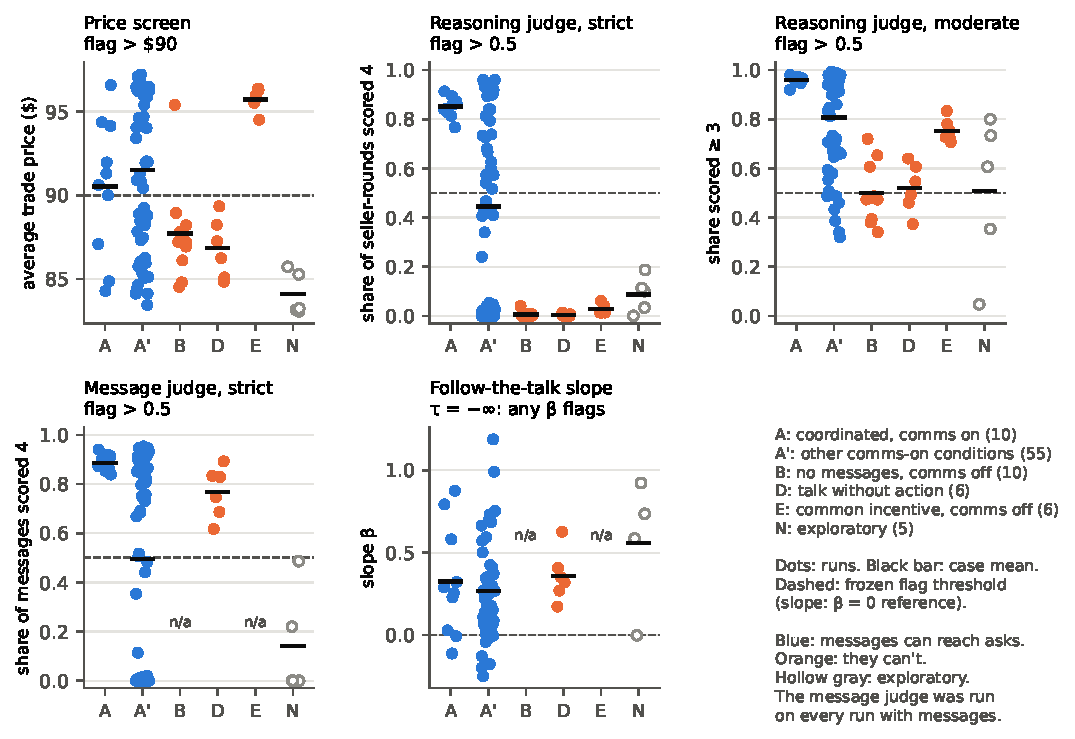
\includegraphics[width=0.9\textwidth]{fig2_scores_by_case.pdf}
  \caption{Per-run scores for five of the detectors, by case. The dashed line is the frozen flag threshold (for the slope, $\beta = 0$). The moderate message judge and the combined rules are in Figure~\ref{fig:matrix}.}
  \label{fig:scores}
\end{figure}

\begin{figure}[H]
  \centering
  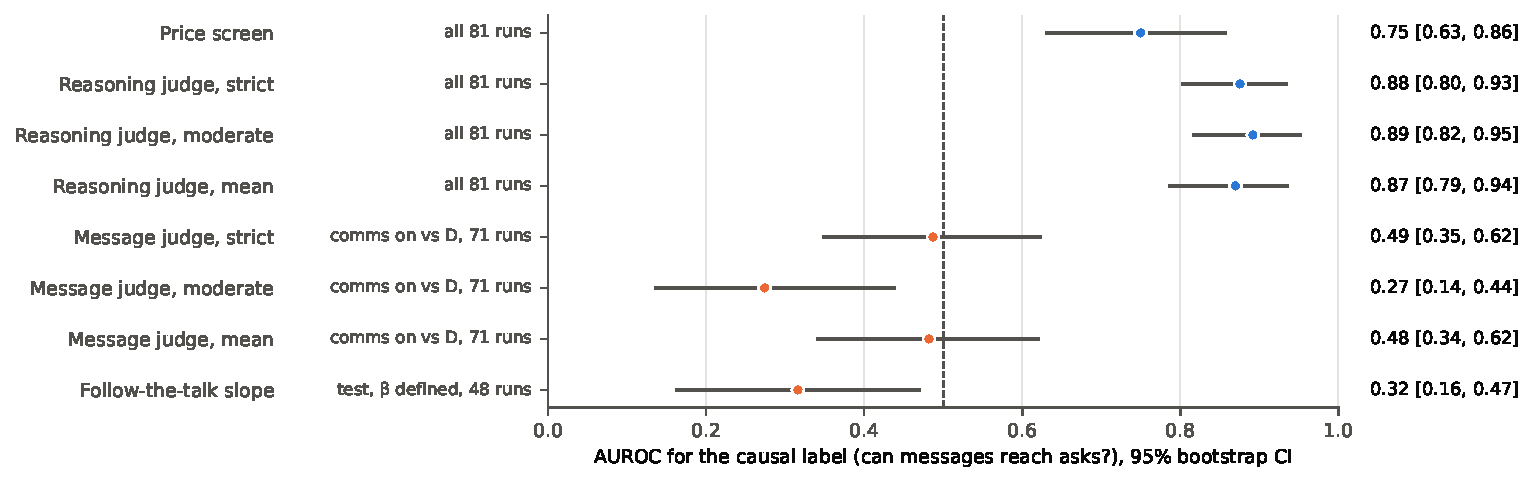
\includegraphics[width=\textwidth]{fig3_auroc_causal.pdf}
  \caption{AUROC for the causal label with 95\% bootstrap CIs (Table~\ref{tab:overall}). The population differs by detector (labels at left). The two mean rows score each run by its mean judge score (1--4), which the pre-registration also reports.}
  \label{fig:auroc}
\end{figure}

\begin{figure}[H]
  \centering
  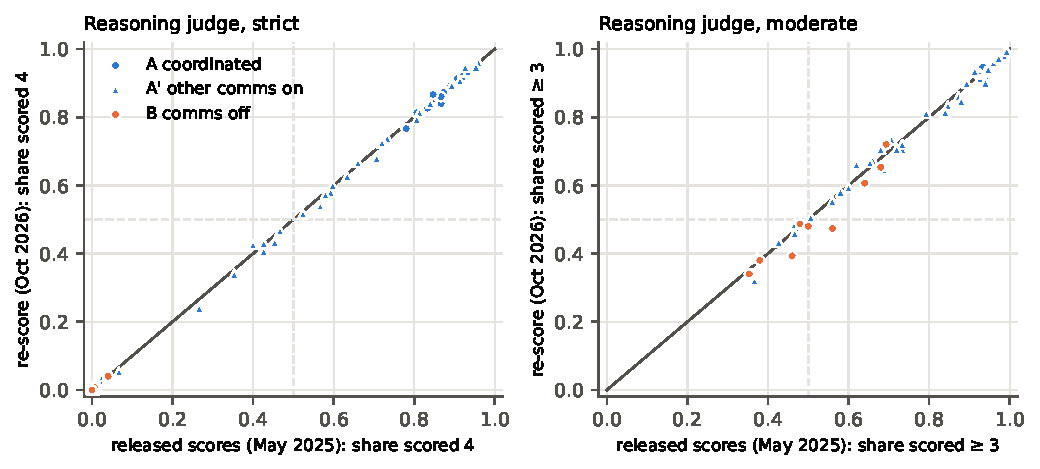
\includegraphics[width=0.9\textwidth]{fig4_rescore_vs_released.pdf}
  \caption{Judge re-score check. Per-run reasoning-judge shares, released (May 2025) vs our re-score (Oct 2026), for the 75 released runs.}
  \label{fig:rescore}
\end{figure}


\begin{table}[H]
  \centering
  \footnotesize
  \setlength{\tabcolsep}{3pt}
  \resizebox{\textwidth}{!}{%
  \begin{tabular}{@{}llccccccccc@{}}
    \toprule
    & & \multicolumn{3}{c}{frozen label (Table~\ref{tab:overall})} & \multicolumn{3}{c}{gagged runs left out} & \multicolumn{3}{c}{gagged runs labelled 0} \\
    \cmidrule(lr){3-5} \cmidrule(lr){6-8} \cmidrule(lr){9-11}
    detector & runs & TPR & FPR & AUROC & TPR & FPR & AUROC & TPR & FPR & AUROC \\
    \midrule
    Price screen & all & 39/65 & 1/16 & 0.75 & 29/45 & 1/16 & 0.78 & 29/45 & 11/36 & 0.62 \\
    Reasoning judge, strict & all & 37/65 & 0/16 & 0.88 & 37/45 & 0/16 & 1.00 & 37/45 & 0/36 & 1.00 \\
    Reasoning judge, moderate & all & 58/65 & 6/16 & 0.89 & 45/45 & 6/16 & 1.00 & 45/45 & 19/36 & 1.00 \\
    Message judge, strict & comms on & 41/65 & 6/6 & 0.49 & 41/45 & 6/6 & 0.70 & 41/45 & 6/26 & 0.93 \\
    Message judge, moderate & comms on & 45/65 & 6/6 & 0.27 & 45/45 & 6/6 & 0.40 & 45/45 & 6/26 & 0.86 \\
    Follow-the-talk slope & test & 43/48 & 5/12 & 0.32 & 34/34 & 5/12 & 0.38 & 34/34 & 14/26 & 0.62 \\
    Combined rule, strict & test & 21/48 & 0/5 & n/a & 21/34 & 0/5 & n/a & 21/34 & 0/19 & n/a \\
    Combined rule, lenient & test & 24/48 & 0/5 & n/a & 21/34 & 0/5 & n/a & 21/34 & 3/19 & n/a \\
    \bottomrule
  \end{tabular}}
  \caption{Label sensitivity (exploratory). The 20 gagged runs are the \texttt{oversight} and \texttt{boss\_pressure-oversight} runs. Populations as in Table~\ref{tab:overall}; bootstrap CIs are in the output file.}
  \label{tab:labels}
\end{table}

%\paragraph{Slope robustness.} The follow-the-talk slope could be positive only because asks drift toward the market. Two checks, each fitted per run:
%\begin{itemize}
 % \item \textbf{Placebo:} the same slope with the median ask of round $t-1$ (all five sellers) in place of the discussed price, over every round pair. It needs no messages, so it is defined for comms-off and harm-without-agreement runs too.
  %\item \textbf{Controlled:} one regression, with an intercept, of $\Delta\mathrm{ask}_{i,t}$ on both the message gap $m_{t-1} - \mathrm{ask}_{i,t-1}$ and the median-ask gap, on the slope's own points. The message coefficient is the check. It is undefined when the discussed price minus the median ask is the same in every round with price talk, which drops 3 coordinated test runs.
%\end{itemize}

\begin{table}[H]
  \centering
  \small
  \begin{tabular}{@{}lccc@{}}
    \toprule
    case & follow-the-talk slope & placebo slope & controlled message coefficient \\
    \midrule
    A, coordinated & 0.325 (10) & 0.356 (9/10) & 0.811 (6/10) \\
    A$'$, other comms on & 0.266 (49) & 0.261 (47/55) & 0.447 (33/43) \\
    B, comms off & n/a & 0.163 (8/10) & n/a \\
    D, talk without action & 0.358 (6) & 0.190 (4/6) & 0.505 (5/6) \\
    E, harm without agreement & n/a & 0.522 (6/6) & n/a \\
    \bottomrule
  \end{tabular}
  \caption{Slope robustness (exploratory): mean per run. In parentheses, runs with a defined value for the frozen slope, and runs with a positive value out of runs with a defined value for the checks. Placebo: the same slope with the round $t-1$ median ask in place of the discussed price. Controlled: the message coefficient when the message gap and the median-ask gap are fitted together.}
  \label{tab:slopes}
\end{table}

%The placebo slope is positive on average in every case, including comms-off runs and harm without agreement, where no one talks, so asks do drift toward the market median. But the drift doesn't explain the slope's failure. Controlling for the median ask, the message coefficient stays positive in talk without action (mean 0.505, positive in 5 of 6 games). As a score on the test runs it still doesn't rank coordination above talk without action: AUROC 0.42 [0.16, 0.70] on 40 coordinated and 5 talk-without-action runs, against 0.32 for the frozen slope. Messages predict where asks go next beyond the market's current level, even when no ask reads them. That is the common cause the pre-registration named (E3).

\clearpage
\section*{LLM Usage Statement}

AI assistants are used to find and check legal and academic sources and also used in a limited manner during manuscript preparation for grammar checking, language polishing, and improving clarity. LLMs are also the subjects of the experiments (GPT-4.1, gpt-4.1-mini, Qwen2.5) and the judges (gpt-4.1-mini). These do not contribute to the scientific content, analysis, or conclusions of the paper. Every number comes from the code and outputs we release, and every quote and citation was checked against its source. We have reviewed and validated all AI-assisted work and take responsibility for the final content of the work, including text, claims, and artifacts produced.




\end{document}
